\section{FOUNDATIONS OF VEDIC ASTROLOGY}
 
\subsection{\textbf{Introduction to the Foundations of Vedic Astrology by Vamadeva
From Planets, Signs and Houses to Aspects, Planetary Periods and Yogas}}

 

\subsection{PART I. THE BACKGROUND OF VEDIC ASTROLOGY, THEORY AND CALCULATIONS}
 

We begin with setting forth the right spiritual and philosophical background for Vedic Astrology, the foundation of yogic thought and yogic living necessary to makes us into proficient Vedic astrologers. This is the basis of Rishi Astrology as opposed to merely personal astrology. It explains the basis of Vedic Astrology relative to our current culture, referring back to the Vedic world view. It provides the system of Vedic astrology a deeper mystical, philosophical and scientific context, which is necessary for making the purpose of Vedic Astrology clear to the mind and intellect. Vedic Astrology is part of a culture of Yoga and a greater system of Vedic spiritual sciences, including Yoga, Vedanta, Vastu, Sanskrit and Vedic philosophy. Without understanding these connections, Vedic Astrology cannot be properly used or understood (note Astrology of the Seers pages 12-23). So we must introduce Vedic Astrology in its broader Vedic context to understand and apply it properly. Vedas are not just specific mantric texts from the ancient sages of India, they represent an understanding of the cosmic mind, cosmic law and our development as a soul.

 

Vedic astrology is rooted in the Vedic, Yogic and Vedantic view of life and the universe and depends upon it for its calculations and interpretations. It reflects the law of karma, the process of rebirth, and the need of the embodied soul to evolve in consciousness as our primary life goal or dharma. It sees the stars and planets as focal points of Divine Energy and Consciousness to guide us in life as well as to map out our karma. As such it is not just a system of calculation but a philosophy and way of life.

 

Vedic knowledge takes a different view of the world than modern science or than Western astrology. Such different values, different philosophy and psychology must be borne in mind while approaching the technical factors of Vedic astrology and understanding their application.  Vedic astrology also views human history and human civilization in a different light than our modern education, with the vision of the great gurus and yogis, that must be appreciated as well to understand our human purpose. In the Vedic view we live in a Self-aware Conscious Universe. Astrology is an integral part of it and shows the connection between its forces at different levels, dimensions and worlds or lokas. We must experience Vedic astrology within ourselves.

 

\subsubsection{Spiritual Background of Vedic Astrology}
 

Time, called Kala in Sanskrit, is not a mere abstract field of physical forces, but is endowed with subtle energies and rhythms according to cosmic influences and various times cycles or yugas, from the day, month, year, to longer planetary cycles and cosmic cycles of many billions of years. These cosmic time cycles affect us at both individual and collective levels. Vedic astrology sees the planets as powers of cosmic consciousness and intelligence that guide our karma and can help us properly understand, manage and transcend our karma to higher powers of light. This requires that we approach the planets with respect as representing powers of Cosmic Consciousness. Note the nature of time according to Vedic thought. (Astrology of the Seers 6-8).

 

Time itself or Kala is also Maha-Kala or Lord Shiva, who is also the deity of eternity. Ma Kali is his consort and Shakti or power of time. The Vedic Gods or Devas, such as described in yogic and Vedic through, as powers of cosmic intelligence relate to the planets as cosmic powers of time. That is why we look at the planets as deities or Devatas in Vedic astrology. It is part of a spiritual science of time, not mere worship of the literal planets. Time is the dominant cosmic force that rules over our lives and the universe as a whole. Time creates the Cosmic Prana or life force which is the basis of all other energies, both animate and inanimate. This Cosmic Prana moves according to the forces of karma universal, collective and individual levels. Astrology reflects the Cosmic Prana and its karmic movement.  Astrology is a science of karma, not just an outer science. It presumes an intelligent order to the universe, dispensed on all levels.The planets represent the cosmic influences or deities governing our lives and the movement of time and karma, not just certain planets in the solar system (Astrology of the Seers 9-12). The planets are conduits for broader cosmic forces beyond those of our solar system and apply these at the level of our solar system. They represent the prime principles and powers or tattvas of the entire universe in our local manifestation.

 

Western tropical and Vedic sidereal astrology differ on how the signs are calculated, though the signs in both instances have the same basic meanings in terms of qualities and planetary connections in terms of rulership. “Sidereal” refers fixed star based zodiac as in the Vedic zodiac, which is measured by certain points in the fixed stars. “Tropical” astrology refers to an equinox based as in most western astrology, which is no longer aligned with the fixed stars, a situation that occurred around two thousand years ago. Note Astrology of the Seers 25-30. Astronomically the difference between these two zodiacs is around 24 degrees or approaching one full sign. The sidereal zodiac is preferred in Vedic Astrology because of its connection with the fixed stars and through them with the greater cosmic order.

 

In summary, sidereal astrology measures the zodiac relative to the fixed stars, while tropical astrology measures the zodiac relative to the shifting positions of the equinoxes. We must understand their different calculations. We cannot see the tropical zodiac in the sky. It is a mathematical abstraction based upon the equinoxes that are points of Sun-Earth connection only. We can only see the sidereal zodiac in the or zodiac of the fixed stars in the sky.

 


\subsubsection{Tropical and Sideral Zodiacs – Ayanamsha}
 

We must remember that the term “astrology” means “that which relates to the stars”. This implies that only a sidereal astrology based upon the actual stars is a true astrology or science of the stars. The tropical zodiac commonly used in the West is based upon a seasonal division and does not directly relate to the fixed stars. It bases its signs upon the solstices and equinoxes, the points of which are slowly moving background in the zodiac over a 25,000 year period. Clearly, astrology began historically with astronomy as an observation of the stars and planets from actual looking at the sky, and so should be sidereal in basis. There has been much historical debate on this topic, with some scholars proposing that astrology was tropical from its origins, which we cannot accept. We hold that Vedic astrology reflects the original zodiac of the fixed stars. A tropical zodiac is not observable in the heavens as it is a mathematical abstraction. Originally astrology was obviously based upon observing the fixed stars, not on abstract calculations. We can easily note this as the signs of the zodiac or constellations were originally sidereal in nature, marking certain groups of stars.

 

A Vedic Astrologer should be able to explain what the Ayanamsha or the difference of degrees between the two systems (tropical and sidereal zodiacs) is and how to calculate it. He or she should know the different Ayanamshas that are commonly in use today (like Raman and Lahiri or Fagan-Bradley, Astrology of the Seers 31-33). People in the West tend to identify astrology with the tropical signs and do not understand that these tropical signs, as used in Sun signs of western astrology, no longer reflect actual astronomical positions. We may need to be able to clarify this to people coming from a background of western astrology. Many people still consider that the tropical zodiac is observable, when it actually was based upon stellar positions of two thousand years ago. It has replaced these with a division of time based upon the equinoxes that no longer reflects the actual stars.

 

The Vedic Ayanamsha reflects the fixed star point of 0 Aries, while the tropical zodiac uses the point of the vernal equinox for 0 Aries. The difference between the two is now around 24 degrees, with the actual vernal equinox occurring around 6 degrees of Pisces. There are some different Ayanamshas reflecting different opinions on where this 0 point of Aries is exactly located. It is often calculated 180 degrees opposite of the point of the start Chitra (Spica) which is regarded to mark the point of 0 Libra in Vedic astrology. But there are other Ayanamsha calculations that vary it from this point slightly, usually by one or two degrees. So the differences in Ayanamsha calculation are relatively minor.

 

For easy calculation purposes with existing western astrology charts, we can take any existing tropical chart and turn it into a sidereal chart by subtracting the appropriate Ayanamsha amount from all planetary positions. This will take most positions back into the previous sign, as the different between the two zodiacs is around 24 degrees according to the most commonly used Lahiri Ayanamsha. As the Ayanamsha is a technical point, we will discuss it in other contexts as well. Vedic software programs allow us to choose the Ayanamsha that we prefer for chart calculations.

 

Note the following article for those interested in the esoteric orientation of the Vedic view of the Zodiac relative to the Milky Way:

The Shiva-Kali Axis in Vedic Astrology \\
 \url{https://www.vedanet.com/the-shiva-kali-axis-in-vedic-astrology-and-its-alignment-in-2020/}

\subsubsection{The Yugas or World Ages}
 

Vedic astrology reflects a different view of time, life and history than modern science or western religions. It emphasizes how natural time is connected with cosmic energies. It sees time cycles, both nature and historical, in terms of yugas or world-ages. The Vedic view of human history reflects astronomical time-cycles and their effect upon human life. This spiritual view of history differs radically from that of history as we generally know it through modern science as it considers esoteric knowledge, and the connection of life on Earth with other domains of the universe.

 

The Vedic view of time is not the same as that of history text books. The Vedic view is that humanity is governed by longer astronomical cycles, and that our current civilization is neither the first, nor the highest – with consciousness pervading the entire universe, not merely a creaturely phenomenon. Unless we recognize and respect these cosmic time cycles, it will be difficult for us to understand the karmic circumstance of our lives or our society. The four Yugas, as taught by Sri Yukteswar in his Holy Science, guru of Paramahansa Yogananda, are given in the Astrology of the Seers and their importance explained. Astrology governs both individual and collective karma. Once we understand this fact, we will have great respect for what astrology indicates, including its usage for understanding collective karma and political events. Yet one may learn Vedic Astrology even if one does not accept or emphasize the Yukteswar theory of the Yugas or any other current Yuga theories.

For those interested in more details on this topic, note this online article by Dr. Frawley:

Keys to the Yugas or Cycles of the Ages in the Sri Yukteswar Yuga Cycle
Keeping this philosophical background in mind, we will now go into the actual prime factors of Vedic astrology, starting with the planets, which are the most important.

 
\subsection{1. THE NINE PLANETS (NAVAGRAHA)}
 

The nine planets of Sun (Surya), Moon (Chandra), Mercury (Budha), Venus (Shukra), Mars (Kuja), Jupiter (Brihaspati, Guru), Saturn (Shani), Rahu and Ketu are the main factors in Vedic astrology.

 

If you can understand the planets, you can easily understand all the rest of Vedic astrology. Vedic astrology is a science of understanding planetary influences. Other astrological factors like signs and houses develop out of these. We are just introducing the planets here and will explain them in greater detail and different levels in other parts of the course. We have again listed some supplementary reading from Astrology of the Seers, in which these points are also discussed.

Note the upcoming lesson on Planetary Types in Lesson 5 for an extensive delineation of  PLANETARY TYPES, in which the qualities of the planets on various levels will be discussed and synthesized. In this lesson we are introducing their basic indications, which will be supplemented later

Note that traditional Vedic astrology does not use Uranus, Neptune and Pluto, though some Vedic astrologers do. Rahul and Ketu are not actual planets but eclipse nodes that have a secondary planetary nature in Vedic thought, but are very important.

 

\subsubsection{THE PLANETS: THE GREAT COSMIC SIGNIFICATORS (Astrology of the Seers, Chapter 4, pages 47-55)}

\subsubsubsection{PLANETS AND THE THREE GUNAS}

 

The nine planets relate to the three primary qualities or gunas of Sattva, Rajas and Tamas, Nature’s prime qualities of harmony, movement and inertia, which is  part of their natural status. These three qualities make up Prakriti, the Vedic terms for the essential energy of Nature.

 

Vedic knowledge systems aim at promoting sattva guna as the power of balance and higher awareness as the factor of growth for the mind and the soul. Rajas or the quality of action is reflecting more in our sense and motor organs along with our emotional impulses. Tamas or the quality of inertia is reflected in the body and the forces that pull us down in life, like gravity. We must consider these three forces relative to the planets as well.

\begin{enumerate}
\item[*] Sattvic Planets that promote awareness, harmony, intelligence, balance – Sun, Moon, Jupiter
\item[*] Rajasic Planets that promote action, expression, movement, change  – Mercury, Venus
\item[*] Tamasic Planets that develop inertia, resistance, opposition, obstruction – Mars, Saturn, Rahu, Ketu
\item[*] There is some crossover of this information with  benefic and malefic status discussed below. Malefic planets are tamasic, except the Sun. All benefic planets are either sattvic or rajasic.
\end{enumerate}
 

\subsubsubsection{PLANETS AND THE FIVE ELEMENTS}

 

The planets relate to the five elements of Earth, Water, Fire, Air and Ether as part of their natural status. The Five Elements are one of the key concepts in Vedic thought and have several levels of applications relative to the planets and signs, as well as on other levels. For example, they also relate to the five lower chakras of yogic thought and to the structure and function of the physical body in Ayurvedic medicine.The five elements have psychological and spiritual indications, not just physical connections. The five elements form the basic vibratory levels of all existence of matter, life and mind. They are also fields of acting as Earth and work, water and emotion, fire and will, air and thought, space and awareness.

 

\begin{enumerate}
\item[*] Earth – Mercury: allows us to deal with the earth element, though in itself is more airy
\item[*] Water – Moon: Venus: promote watery tendencies physically, emotionally and spiritually
\item[*] Fire – Sun, Mars: develop fire, aggression, assertion, perception
\item[*] Air – Saturn: causes instability, ungroundedness, separation
\item[*] Ether – Jupiter: promote expansion, harmony and ascension
 \end{enumerate}

Some planets consist of the same element but have different gunas (like the Sun as relating to the fire element and sattva guna, with Mars as fire and tamas). The Sun promotes spiritual knowledge, health and well-being, while Mars tends to be impulsive and caught in eventual inertia.

 

Some planets consist of the same gunas but different elements (like Mars and Saturn as tamas in gunas but as fire and air in elements respectively, which both can be destructive). No two planets are the same in terms of both elements and gunas. This helps us determine their unique characteristics.

 

The gunas and elements of the planets fit in with the basic nature and character of the planets. Yet take this information as general guidelines, not as the last word on the planets. Planets are also influenced by the elements of the signs in which they are located and which they rule.

 

\subsubsubsection{PLANETS AS BENEFIC OR MALEFIC/NATURAL STATUS }

 

Vedic astrology designates planets as benefic (supportive or growing in action) or malefic (obstructive or limiting in action), which characterizes their influences and functions overall. This is perhaps their most important distinction that should always be carefully remembered and considered. It should not be taken literally as good or bad, much less good or evil, but as expansive and contractive, supporting or negating. It is not a question of morality or religion but of the working out of energies. Note the main factors below.

 

\begin{enumerate}
\item[*] The Sun is a natural malefic as by its power of heat and light tends to damage the houses and planets it gets associated with in the chart. Its action is powerful but can be harsh. It tends to overpower the other planets.
\item[*] The Moon is a natural benefic as it has a nourishing, cooling and softening effect wherever it is placed, but note that the Moon loses its benefic power to some degree when new or waning.
\item[*] Jupiter is the greater benefic and the most positive planet in the chart for promoting growth, expansion, success, health, knowledge, and fulfillment of karmic goals on all levels.
\item[*] Saturn is the great malefic, opposite to Jupiter in qualities, the most negative planet overall, promoting decline, contraction, defeat, disease and difficult karmas, making us let go or renounce.
\item[*] Venus is the lesser benefic and also has a positive, expansive and creative effect like Jupiter, but with a softer, gentler and more sensitive quality.
\item[*] Mars is the lesser malefic and also has a destructive, divisive and negative effect like Saturn, like its power of fire.
\item[*] Mercury is benefic, supportive and communicative in its own nature, but easily comes under the influence of the planets it is associated with and can thereby change its nature by association, becoming malefic with malefic planets (except with the Sun which it is commonly connected to).
\item[*] Rahu, the north node of the Moon, is much like Saturn as a malefic and disintegrating force but more subtle and psychic in its actions, including more devious and hard to predict.
\item[*] Ketu has a similar malefic influence as Mars but more subtle in its actions, negative and potentially destructive or transcendent, with a strong point focus.
\end{enumerate}

Note that benefics planets are not always good in their effects in the chart, in that benefics promote the powers of the houses that they rule – which can be problematical if these are difficult houses (like 6, 8 or 12, which cause loss and destruction). Similarly, malefics can be good in the chart, in that they can destroy the negative influences of negative factors that they may influence, like negating the factors of disease. So interpretation must be nuanced accordingly.

 

House locations also matter relative to benefics and malefics, whether their effects are overall good or bad for the chart and in what way. We will explore this in detail later. As an important general rule that we frequently emphasize; benefics are good when located in angles and trines (houses 1, 4, 5, 7, 9, 10), while malefics are good in upachaya houses (3, 6, 11 and sometimes 10). This is the most basic rule of planetary location in Vedic astrology, and should never be overlooked.

 

\subsubsubsection{PLANETS IN TERMS OF QUALITIES AND CHARACTERISTICS} (Astrology of the Seers, Chapter 5, Description of the Planets, pages 57-86)

 

Note the Detailed Description of the Planets in this Chapter.

 

Each planet in addition to these general categories just explained has its own unique qualities and characteristics, including the two lunar nodes, Rahu and Ketu. You must understand the range of meaning of each planet, which is extensive. Each can function on a lower and mundane level or on a higher spiritual level. The planets as an all-encompassing symbolism have their counterparts for all processes in life and all levels of consciousness. Note the meaning of the planets and their different qualities of energy:

 


\begin{enumerate}
\item[*] The Sun as the largest and brightest heavenly body represents authority, the king or ruler, leader, father, success, power, prana, will-power, ego, soul and Self.
\item[*] The Moon represents the female ruler, queen, mother, public influence, fertility, creativity, mind, emotions and feelings. It is the fastest moving and most variable of the planets and so its influences change quickly.
\item[*] Mars has a similar fiery energy to the Sun but reduced and specialized as the son, brother, prince, male energy, prowess, aggression, competition, legal and military factors.
\item[*] Venus as the brightest star morning or evening has a similar energy to the Moon but reduced and specialized as the daughter, wife, female energy, attraction, beauty, inspiration, art, luxury, and adornment.
\item[*] Jupiter as the brightest star in the night sky indicates cosmic energy, law, dharma, religion, spirituality, education, wealth, prosperity, abundance, wellbeing and health.
\item[*] Mercury as close to the Sun but of diminished brightness indicates the child, intellect, perception, knowledge, prana, speech, commerce and communication.
\item[*] Saturn as the slowest moving of the planets indicates destiny, time, karma, obstruction, inertia, poverty, disease, longevity, detachment and renunciation.
\item[*] Rahu as the north lunar node indicates illusion, desire, the media, Maya, expansion, deception, notoriety and dissolution.
\item[*] Ketu as the south lunar node indicates perception, research, spiritual knowledge and inquiry but as related to Mars energy also death, termination, injuries, negation.
\end{enumerate}

Each planet functions is interrelated with the others and reflect upon each other. Sun and Moon complement each other as father and mother, active and receptive. Moon and Saturn are opposite in qualities as fast and slow moving planets, affording them a difficult interaction. Jupiter and Saturn are opposite in the way of being expansive or contractive. Jupiter and Mercury represent the mental attributes of broad comprehension versus focused perception. Venus and Mars are opposite as female and male energies. Rahu and Ketu are opposite as the expansive versus contractive forces of collective karma.

Gradually become intimate with planetary meanings on all levels and begin to look at life through the nine windows of the nine planets. Learn to see thee primary factors in the chart that each planet indicates, as well as their variations. The more you understand the planets and their interactions, the more you will understand Vedic astrology. All other complicated factors go back to the planets.

 

\subsection{2. THE TWELVE SIGNS OR RASHIS} (Astrology of the Seers, Chapter 6, the Houses: Domains of Planetary Action, pages 87-110)
 

The twelve signs of the zodiac – Aries, Taurus, Gemini, Cancer, Leo, Virgo, Libra, Scorpio, Sagittarius, Capricorn, Aquarius, Pisces – determine the fields of activity for the planets that rule over them. Each has its own characteristics, qualities and energies reflecting those of their ruling planets.

 

Planets are moving forces, while signs are fixed fields of their operation. The signs are prime factors in Vedic astrology that must be carefully understood, which means understanding their ruling planets. While the Vedic signs have the same names as in western astrology, remember that their calculation is different. Their qualities are similar to those of tropical astrology but with some variations. The signs are called Rashis in Sanskrit which refers to an allotment or calculation, showing their karmic connections.

 

The signs relate to cosmic evolution and the different portions of the cosmic person as time personified (Kala Purusha). As such the twelve signs provide a blueprint for the working out of forces on all levels, whether individual or collective. Be able to articulate through a short description the meaning and characteristics of each of the twelve signs, particularly as rising signs (Ascendants), which is where their main qualities are in evidence. You will need to be able to explain this to your clients. We will explore the 12 Ascendants  in detail in a separate lesson.

 

Each planet rules two signs of the zodiac, except Sun and Moon that rule one.


\begin{enumerate}
\item[*] Aries and Mars, Taurus and Venus, Gemini and Mercury, Cancer and Moon, Leo and Sun, Virgo and Mercury
\item[*] Libra and Venus, Scorpio and Mars, Sagittarius and Jupiter, Capricorn and Saturn, Aquarius and Saturn, Pisces and Jupiter
 \end{enumerate}

The signs reflect the meaning of the planets that rule them. They are fields created by their ruling planets and are best understood according to the characteristics of their ruling planets. Aries, for example, as a Mars ruled sign, reflects Mars energies in its indications and operation.

Become conversant with the signs as expressions of the planets and as twelve windows on life, a blueprint for the twelve phases or twelve aspects of any aspect of life. Learn to be able to explain the basic meanings and indications of each sign.

 

\subsubsection{SIGN QUALITIES }(Astrology of the Seers 89-91)

 

The signs have three overall qualities or energetic orientations:

 

Cardinal (moveable, chara) for Aries, Cancer, Libra and Capricorn
Fixed (sthira) for Taurus, Leo, Scorpio and Aquarius
Mutable (dual, dvisvabhava) signs for Gemini, Virgo, Sagittarius and Pisces
 

A majority of planets in moveable signs will make a person moveable and active both outwardly and inwardly, usually in a focused direction, but can cause assertion, aggression or instability. Can cause changes in residence or the seeking of new gains in life.

A majority of planets in fixed signs will make a person fixed in their personal traits and in their outer action, providing stability but also inertia and unwillingness to change. the person may be stubborn and unyielding. Outwardly their residence or profession may remain the same and seldom change.

A majority of planets in mutable or dual signs will be sensitive, changing and adaptable, but also wavering and vulnerable, volatile and unpredictable, intelligent but ungrounded. Note that moveable signs relate to the mental planets Mercury and Jupiter.

 

Generally planets in moveable signs are more rajasic (willful and assertive), in fixed signs more tamasic (steady but conservative), and in dual signs more sattvic in qualities (ruled by Jupiter and Mercury, intelligent but sensitive). Should Ascendant, Sun and Moon all be located in signs of the same quality, the effects will be more pronounced/ Over time look at these qualities within yourself, in other people and in different circumstances and see if you can find  correlations with the chart.

 

\subsubsection{SIGNS AND ELEMENTS} (Astrology of the Seers 91-94)

 

Each Sign has one of the Four Elements from Earth to Air.

 

\begin{enumerate}
\item[*] Earth (Taurus, Virgo, Capricorn)
\item[*] Water (Cancer, Scorpio, Pisces)
\item[*] Fire (Aries, Leo, Sagittarius)
\item[*] Air (Gemini, LIbra, Aquarius)
 \end{enumerate}

The elements of the sign are important for delineating the fields of activity for each sign and their different personality characteristics. Yet the elements for the signs are always not identical with the elements of their ruling planets and have their own characteristics and value.

Saturn, Mercury and Venus each rule an Earth sign and and Air sign. Saturn with Capricorn and Aquarius, Mercury with Virgo and Gemini, and Venus with Taurus and Libra. Mars and Jupiter, on the other hand, each rule a fire sign and a water sign. Mars with Aries and Scorpio and Jupiter with Sagittarius and Pisces. This is not the same as the elements that the planets rule by nature.

 

\begin{enumerate}
\item[*] A person with many planets in earth signs will have a lot of activity in the field of the earth, body, nature or the physical world and may be earthly in nature.
\item[*] A person with many planets in water signs will be emotional, feeling oriented, relationship oriented and personal in their interactions.
\item[*] A person with many planets in fire signs will be willful, aggressive, intelligent and assertive.
\item[*] A person with many planets in air signs will be changeable, sensitive, expansive and socially minded.
  \end{enumerate}

Yet do not forget the elements of the planets either and their relationship with the elements of the signs. For example, Mars will do well in Leo, a fiery planet in a fire sign. Venus will usually suffer in Leo as a watery planet in a fire sign.

\subsubsection{THE MEANINGS OF THE TWELVE SIGNS CONTINUED} (Astrology of the Seers 94-103)

 

The signs have an additional twofold quality  as odd and even, active and passive, positive and negative. Odd-numbered signs will generally be more masculine and assertive, while even-numbered signs will be more feminine and response.

 


\begin{enumerate}
\item[*] Odd or masculine signs: Aries, Gemini, Leo, Libra, Sagittarius, Aquarius
\item[*] Even or feminine signs: Taurus, Cancer, Virgo, Scorpio, Capricorn, Pisces
    \end{enumerate}

Note the differences in the signs by the sides (active and passive) of their ruling planet predominant in them (though this is only one factor in comparing sign influences).

\begin{enumerate}
\item[*] Aries as the odd sign 1 for Mars is the positive, active, aggressive sign of Mars gives a more independent Mars energy, while Scorpio as its even sign 8 is its negative, passive, resistant sign and works more behind the scenes.
\item[*] Taurus as the even or feminine sign for Venus will give more feminine, creative and artistic Venus energies and gathering material resources. Libra as the odd or masculine sign for Venus will be more concerned with public, commerce, communication, ideals and politics.
\item[*] Gemini as the odd or masculine sign for Mercury will be more expressive, communicative, extroverted, mathematical, scientific and abstract in its approach. Virgo as the even or feminine sign of \item[*] Mercury will be more feminine, artistic, home oriented, healing oriented and introverted.
\item[*] Sagittarius as the odd or masculine sign for Jupiter will be more expressive, assertive, legalistic, military, judgmental and expansive. Pisces as the feminine sign will be more intuitive, emotional, creative, receptive and nurturing.
\item[*] Capricorn as the even or feminine sign for Saturn will be more public oriented, influenceable, work oriented and adaptable. Aquarius as the odd or masculine sign will be more principled, expansive and intellectual.
   \end{enumerate}

\subsubsection{Combining Qualities and Elements of Signs}

 

We can differentiate the meaning of signs further by their contrasts of qualities and elements. For example, Libra as moveable air is more expressive than Aquarius as fixed air, which is more withdrawn, while Gemini as mutable or dual-natured air, will be more volatile. Cancer as moveable water is more emotional than Capricorn as moveable earth that is more practical.

 

Planets reflect the elements of the signs in which they are located, more so if they share a common element. The element of the Ascendant or rising sign colors the chart as a whole. Planets gain strength if located in signs of similar elements, like the fiery Sun in a fiery sign like Sagittarius. Planets are weaker in signs ruled by an opposite element, like the fiery Sun being weaker in a watery sign like Pisces.

 

Begin to examine the twelve signs and how they relate and how they differ. It is important that we begin to think about these planetary factors ourselves, rather than just rely upon descriptions in books. We must learn to think in terms of Vedic astrology and learn its language. Above all, learn to look into the balance of the energies of the Ascendant, Moon and Sun signs as representing body, mind and character. In this regard signs create a typology of their own. Planetary types are one of the key factors of chart interpretation.

Note that the Workbook Lesson 3 has a special lesson on the meaning of each Sign as an Ascendant Sign. This will help you understand the meaning of the signs. You can look into it for more detail as needed.

 

\subsubsection{Astroart of the Twelve Signs Courtesy of Hinduism Today}
 

Below are some traditional paintings of the signs from India. These reflect their dominant animal symbol and characteristics.

\begin{figure}[H]
 \centering
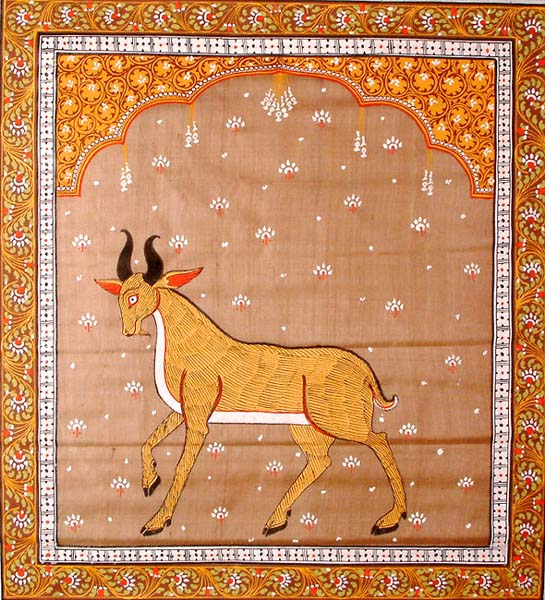
\includegraphics[width=0.5\textwidth]{pics/Aries.png}
 \end{figure}
 

Hindu Drawing of Aries as the Ram
Aries as the Ram is headstrong, assertive, forward movement, determined but obstinate.


 \begin{figure}[H]
 \centering
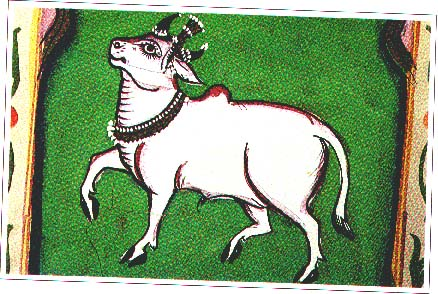
\includegraphics[width=0.5\textwidth]{pics/Taurus.png}
 \end{figure}

Hindu Drawing of Taurus as Bull
Taurus as the bull is strong, steady, creative, earthly and fixed.



 \begin{figure}[H]
 \centering
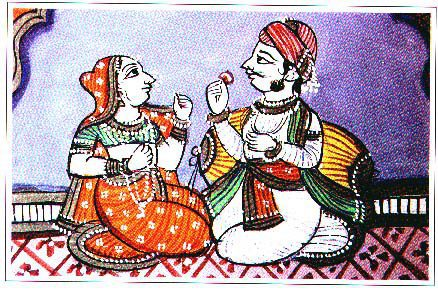
\includegraphics[width=0.5\textwidth]{pics/Gemini.png}
 \end{figure}

Hindu Drawing of Gemini
Vedic astrology regards Gemini as a male and female couple, not as twins as in western astrology.
Gemini is sensitive, volatile, communicative, relationship oriented, ambivalent.

 

\begin{figure}[H]
 \centering
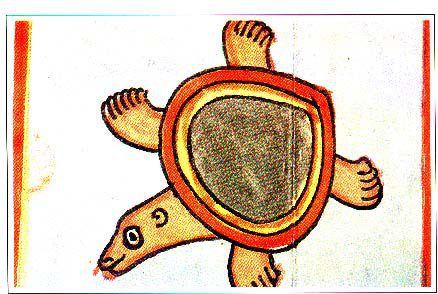
\includegraphics[width=0.5\textwidth]{pics/Cancer.png}
 \end{figure}

 

Hindu Drawing of Cancer as Crab
Cancer as a crab is often hard to understand for the sign of the Moon.
Shows the indrawn nature of lunar emotions but that can also have a power of expression.



 \begin{figure}[H]
 \centering
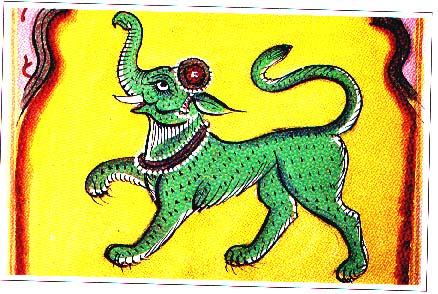
\includegraphics[width=0.5\textwidth]{pics/Leo.png}
 \end{figure}

Hindu Drawing of Leo
Combines Elephant and Lion as sign of Royalty.
Leo is warm, expressive, guiding, leading, but potentially dominating and overpowering.

 
\begin{figure}[H]
 \centering
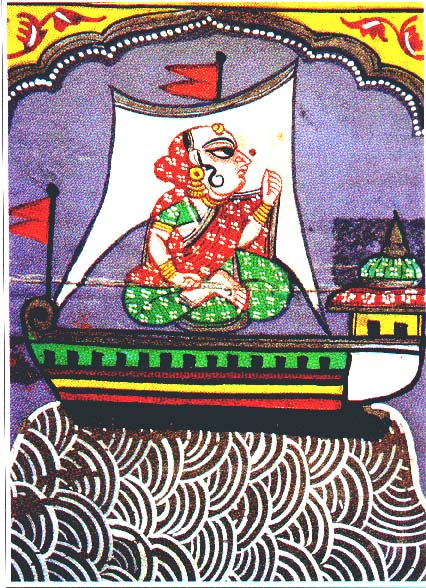
\includegraphics[width=0.5\textwidth]{pics/Virgo.png}
 \end{figure}


 

Hindu Drawing of Virgo
Vedic astrology sees Virgo as a young girl and often a woman overall.
Virgo has both manual and mental skills, is creative, sensitive, vulnerable, yet focused.

 
\begin{figure}[H]
 \centering
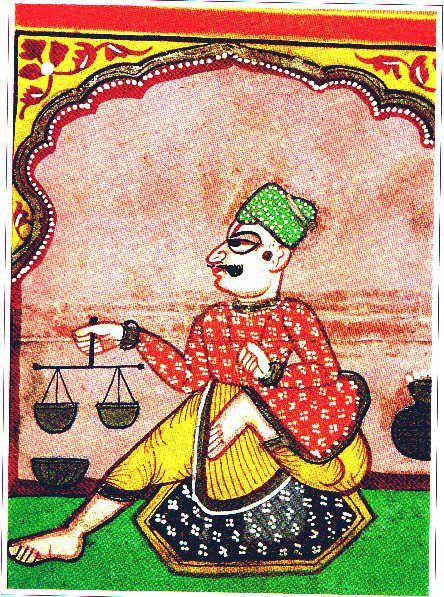
\includegraphics[width=0.5\textwidth]{pics/Libra.png}
 \end{figure}


 

Hindu Drawing of Libra
Merchant Weighing Scales
Libra is concerned with balance, harmony, commerce, communication, both on outer and inner levels.

 

\begin{figure}[H]
 \centering
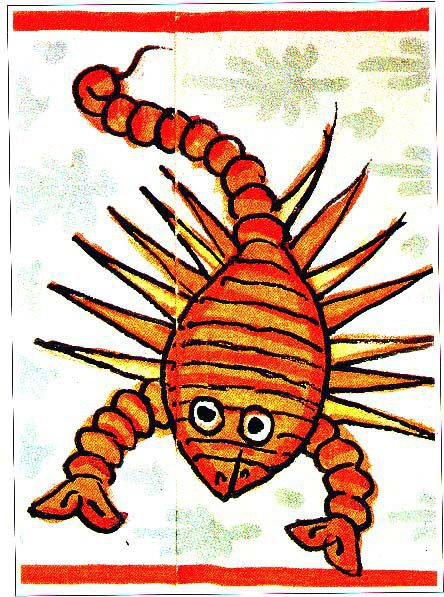
\includegraphics[width=0.5\textwidth]{pics/Scorpio.png}
 \end{figure}

 

Hindu Drawing of Scorpio

Scorpio like the literal serpent has poison in its tail and connects to deep emotional, occult and spiritual energies.


\begin{figure}[H]
 \centering
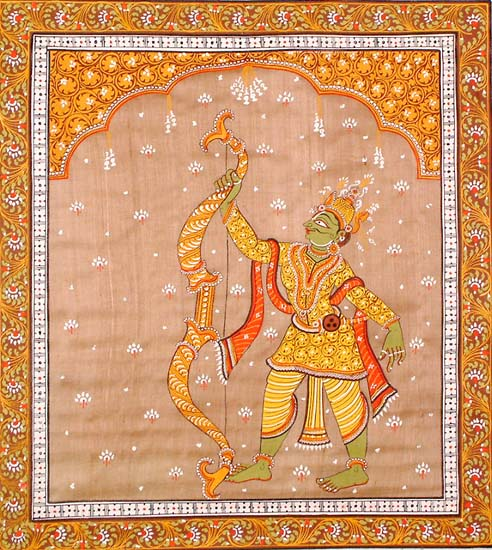
\includegraphics[width=0.5\textwidth]{pics/Sagitarius.png}
 \end{figure}


Hindu Drawing of Sagittarius
As the Bowman
Sagittarius relates to law, dharma, the police, army, gurus, and gives focus.

 

\begin{figure}[H]
 \centering
\includegraphics[width=0.5\textwidth]{pics/Capricorn.png}
 \end{figure}

 

Hindu Drawing of Capricorn
Sometimes a crocodile but other times a mountain goat is used for Capricorn.
Represents the ability to move on Earth and scale its heights but with effort and challenges.

 

\begin{figure}[H]
 \centering
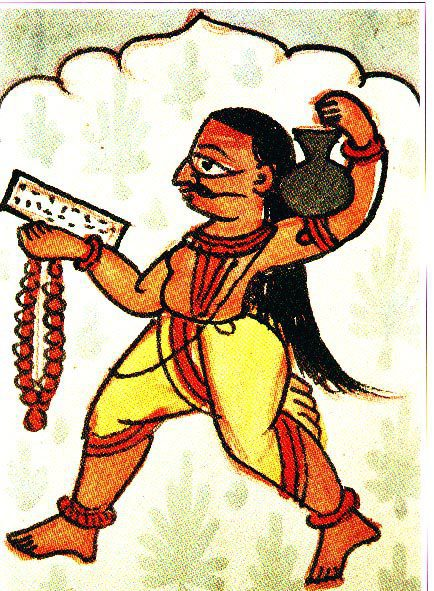
\includegraphics[width=0.5\textwidth]{pics/Aquarius.png}
 \end{figure}

Hindu Drawing of Aquarius
As a man carrying a Water Pot
The water pot is wisdom, the cosmic space, spiritual sensitivity, humanism.

 


\begin{figure}[H]
 \centering
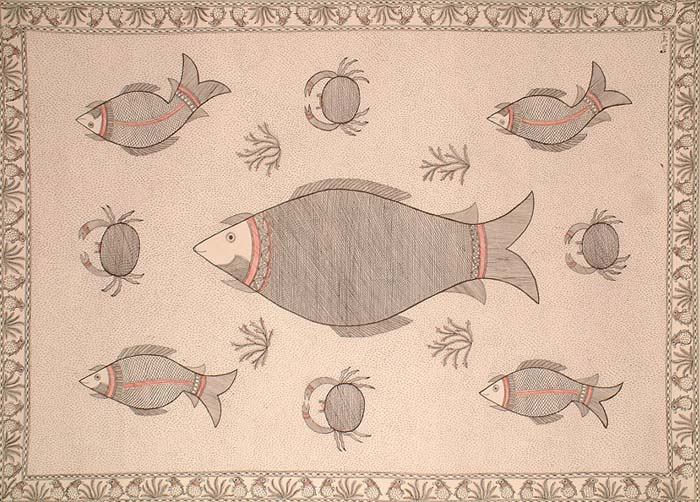
\includegraphics[width=0.5\textwidth]{pics/Pisces.png}
 \end{figure}
 

Hindu Drawing of Pisces as the Fish
The fish indicates absorption, mergence, introversion, intuition and completion.



 

\subsubsection{COURSE WORKBOOK FOR EXAMINATION OF SOUTH AND NORTH INDIAN VEDIC CHARTS}

The course Workbook, which is supplementary to the other three course volumes, is also referred to in these lessons, as we have already noted. It comes after the other three course volumes in the course index. Just scroll down to find it.

For this particular lesson, once you have completed the lesson material, please examine the first lesson of the Workbook, particularly if you do not know how to read North and South Indian charts and their differences, which the Workbook provides examples for. It teaches you how to read both types of charts. 